\documentclass[tikz,border=6pt]{standalone}
\usepackage[T1]{fontenc}
\usepackage[utf8]{inputenc}
\usepackage{pgfplots}
\usepgfplotslibrary{groupplots}
\usetikzlibrary{calc}
\pgfplotsset{compat=1.18}
\begin{document}
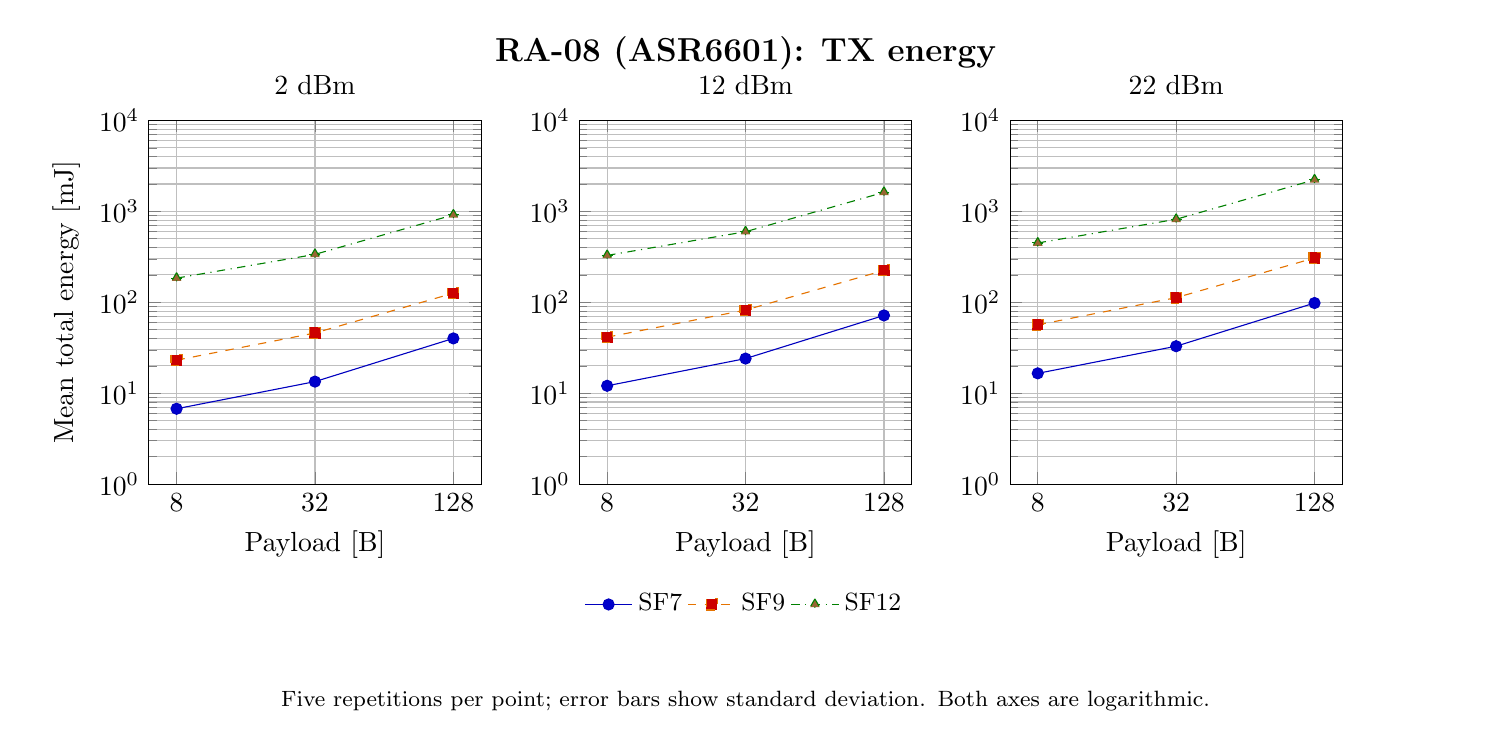
\begin{tikzpicture}
\begin{groupplot}[/pgf/number format/use comma, group style={group size=3 by 1, horizontal sep=1.25cm},
  width=5.8cm,height=6.2cm,xmode=log,log basis x=2,ymode=log,log basis y=10,ymin=1,ymax=10000,
  xtick={8,32,128},xticklabels={8,32,128},grid=both,xlabel={Payload [B]},
  legend style={draw=none,fill=none,font=\small,at={(0.5,-0.27)},anchor=north,legend columns=-1}]
% TX energy
\nextgroupplot[title={2 dBm},ylabel={Mean total energy [mJ]}]
\addplot+[blue!75!black,solid,mark=*,error bars/.cd,y dir=both,y explicit] coordinates {(8,6.73714814) +- (0,0.0020909223) (32,13.3982554) +- (0,0.00304912157) (128,40.0253923) +- (0,0.01240793)};
\addplot+[orange!90!black,dashed,mark=square*,error bars/.cd,y dir=both,y explicit] coordinates {(8,23.064778) +- (0,0.0132317097) (32,45.9096928) +- (0,0.0238317218) (128,125.72722) +- (0,0.0516739042)};
\addplot+[green!50!black,dashdotted,mark=triangle*,error bars/.cd,y dir=both,y explicit] coordinates {(8,184.153955) +- (0,0.0614046943) (32,336.07955) +- (0,0.090116738) (128,913.845509) +- (0,0.262878348)};
\nextgroupplot[title={12 dBm}]
\addplot+[blue!75!black,solid,mark=*,error bars/.cd,y dir=both,y explicit] coordinates {(8,12.0503917) +- (0,0.0247695662) (32,24.0092558) +- (0,0.0729850237) (128,71.620511) +- (0,0.195996517)};
\addlegendentry{SF7}
\addplot+[orange!90!black,dashed,mark=square*,error bars/.cd,y dir=both,y explicit] coordinates {(8,41.2943001) +- (0,0.120029143) (32,82.0669612) +- (0,0.247554931) (128,224.054454) +- (0,0.394304198)};
\addlegendentry{SF9}
\addplot+[green!50!black,dashdotted,mark=triangle*,error bars/.cd,y dir=both,y explicit] coordinates {(8,327.33546) +- (0,0.434639923) (32,596.918749) +- (0,0.913943909) (128,1618.52608) +- (0,2.25498449)};
\addlegendentry{SF12}
\nextgroupplot[title={22 dBm}]
\addplot+[blue!75!black,solid,mark=*,error bars/.cd,y dir=both,y explicit] coordinates {(8,16.5149661) +- (0,0.0215876065) (32,32.8358955) +- (0,0.0946227038) (128,98.0504253) +- (0,0.257586409)};
\addplot+[orange!90!black,dashed,mark=square*,error bars/.cd,y dir=both,y explicit] coordinates {(8,56.4390596) +- (0,0.124893974) (32,112.374425) +- (0,0.23018278) (128,306.862201) +- (0,0.400943568)};
\addplot+[green!50!black,dashdotted,mark=triangle*,error bars/.cd,y dir=both,y explicit] coordinates {(8,448.614794) +- (0,0.656256626) (32,817.933317) +- (0,0.808675368) (128,2223.05304) +- (0,0.965374333)};
\end{groupplot}
\node[font=\bfseries\large] at ($(group c2r1.north)+(0,0.85cm)$) {RA-08 (ASR6601): TX energy};
\node[font=\footnotesize,align=center,text width=18cm] at ($(group c2r1.south)+(0,-2.75cm)$) {Five repetitions per point; error bars show standard deviation. Both axes are logarithmic.};
\end{tikzpicture}
\end{document}
